\documentclass{standalone}
\usepackage{tikz}
\usetikzlibrary{patterns, positioning}


\begin{document}
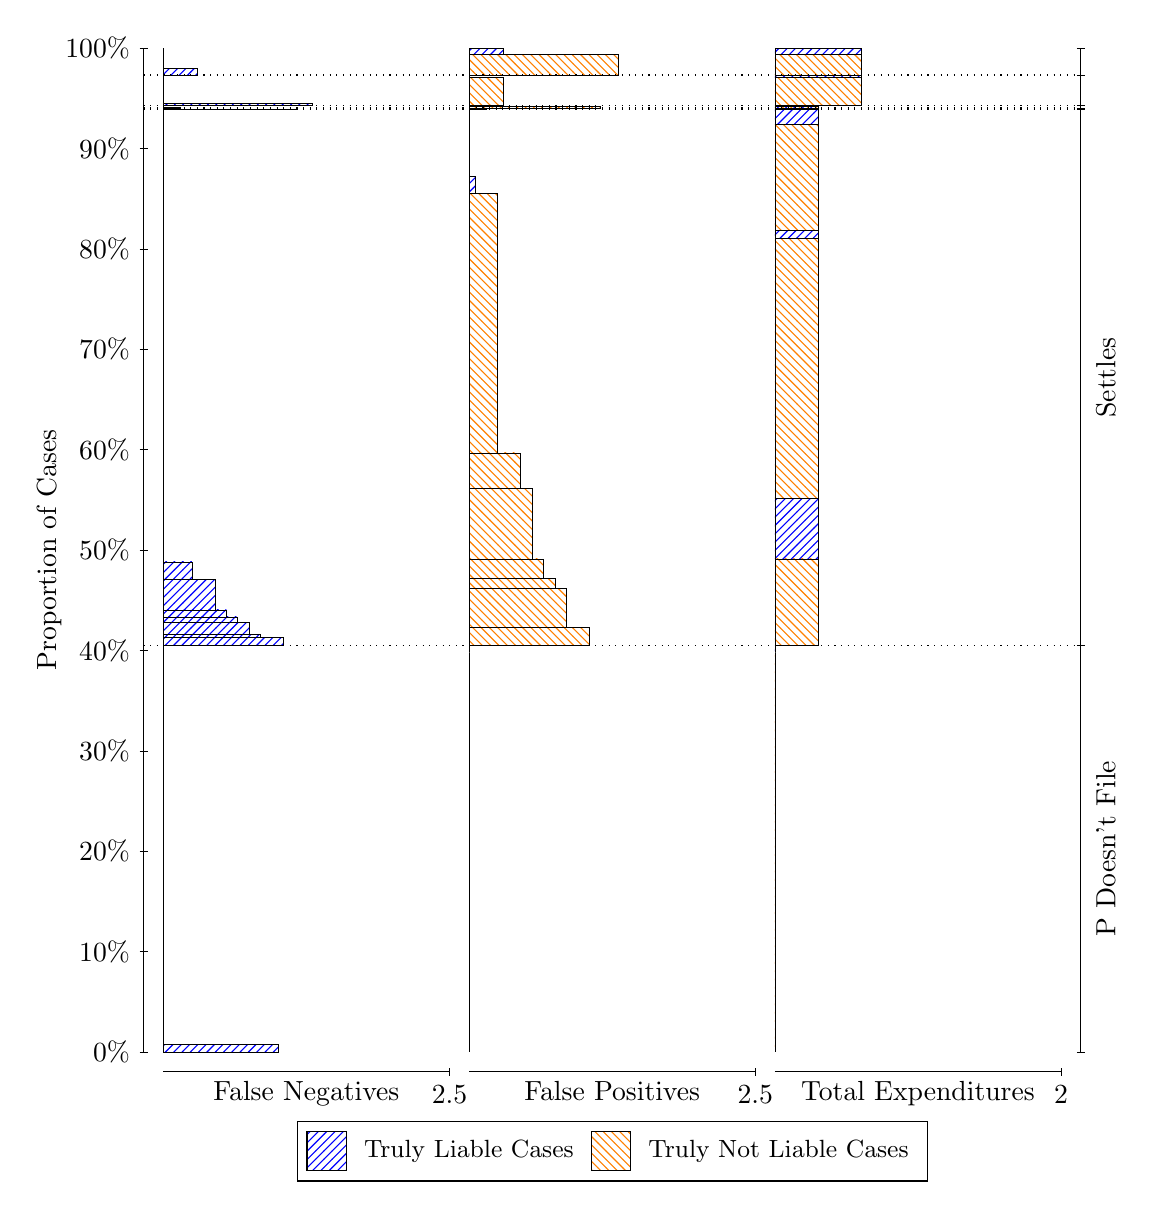
\begin{tikzpicture}
\draw[black, very thin] (1.5,1.75) -- (1.5,14.5);
\node[rotate=90, text=black, anchor=center] at (0.3, 8.125) {Proportion of Cases};
\draw[black, very thin] (1.45,1.75) -- (1.55,1.75);
\node[text=black, anchor=east] at (1.45, 1.75) {0\%};
\draw[black, very thin] (1.45,3.025) -- (1.55,3.025);
\node[text=black, anchor=east] at (1.45, 3.025) {10\%};
\draw[black, very thin] (1.45,4.3) -- (1.55,4.3);
\node[text=black, anchor=east] at (1.45, 4.3) {20\%};
\draw[black, very thin] (1.45,5.575) -- (1.55,5.575);
\node[text=black, anchor=east] at (1.45, 5.575) {30\%};
\draw[black, very thin] (1.45,6.85) -- (1.55,6.85);
\node[text=black, anchor=east] at (1.45, 6.85) {40\%};
\draw[black, very thin] (1.45,8.125) -- (1.55,8.125);
\node[text=black, anchor=east] at (1.45, 8.125) {50\%};
\draw[black, very thin] (1.45,9.4) -- (1.55,9.4);
\node[text=black, anchor=east] at (1.45, 9.4) {60\%};
\draw[black, very thin] (1.45,10.675) -- (1.55,10.675);
\node[text=black, anchor=east] at (1.45, 10.675) {70\%};
\draw[black, very thin] (1.45,11.95) -- (1.55,11.95);
\node[text=black, anchor=east] at (1.45, 11.95) {80\%};
\draw[black, very thin] (1.45,13.225) -- (1.55,13.225);
\node[text=black, anchor=east] at (1.45, 13.225) {90\%};
\draw[black, very thin] (1.45,14.5) -- (1.55,14.5);
\node[text=black, anchor=east] at (1.45, 14.5) {100\%};

\draw[black, very thin] (13.4,1.75) -- (13.4,14.5);
\draw[black, very thin] (13.35,1.75) -- (13.45,1.75);
\node[anchor=west] at (13.35, 1.75) {};
\draw[black, very thin] (13.35,6.9124) -- (13.45,6.9124);
\node[anchor=west] at (13.35, 6.9124) {};
\draw[black, very thin] (13.35,13.717) -- (13.45,13.717);
\node[anchor=west] at (13.35, 13.717) {};
\draw[black, very thin] (13.35,13.739) -- (13.45,13.739);
\node[anchor=west] at (13.35, 13.739) {};
\draw[black, very thin] (13.35,13.768) -- (13.45,13.768);
\node[anchor=west] at (13.35, 13.768) {};
\draw[black, very thin] (13.35,14.157) -- (13.45,14.157);
\node[anchor=west] at (13.35, 14.157) {};
\draw[black, very thin] (13.35,14.5) -- (13.45,14.5);
\node[anchor=west] at (13.35, 14.5) {};

\draw[black, very thin, pattern color=blue, pattern=north east lines] (1.75,1.75) rectangle (3.2033,1.8416);
\draw[black, very thin, pattern color=orange, pattern=north west lines] (1.75,1.8416) rectangle (1.75,6.9124);
\draw[black, very thin, pattern color=blue, pattern=north east lines] (1.75,6.9124) rectangle (3.276,7.0184);
\draw[black, very thin, pattern color=blue, pattern=north east lines] (1.75,7.0184) rectangle (2.9853,7.0537);
\draw[black, very thin, pattern color=blue, pattern=north east lines] (1.75,7.0537) rectangle (2.84,7.2037);
\draw[black, very thin, pattern color=blue, pattern=north east lines] (1.75,7.2037) rectangle (2.6947,7.2745);
\draw[black, very thin, pattern color=blue, pattern=north east lines] (1.75,7.2745) rectangle (2.5493,7.3635);
\draw[black, very thin, pattern color=blue, pattern=north east lines] (1.75,7.3635) rectangle (2.404,7.7562);
\draw[black, very thin, pattern color=blue, pattern=north east lines] (1.75,7.7562) rectangle (2.1133,7.9738);
\draw[black, very thin, pattern color=orange, pattern=north west lines] (1.75,7.9738) rectangle (1.75,13.717);
\draw[black, very thin, pattern color=blue, pattern=north east lines] (1.75,13.717) rectangle (3.4213,13.718);
\draw[black, very thin, pattern color=orange, pattern=north west lines] (1.75,13.718) rectangle (1.75,13.739);
\draw[black, very thin, pattern color=blue, pattern=north east lines] (1.75,13.739) rectangle (1.968,13.748);
\draw[black, very thin, pattern color=orange, pattern=north west lines] (1.75,13.748) rectangle (1.75,13.768);
\draw[black, very thin, pattern color=blue, pattern=north east lines] (1.75,13.768) rectangle (3.6393,13.797);
\draw[black, very thin, pattern color=orange, pattern=north west lines] (1.75,13.797) rectangle (1.75,14.157);
\draw[black, very thin, pattern color=blue, pattern=north east lines] (1.75,14.157) rectangle (2.186,14.24);
\draw[black, very thin, pattern color=orange, pattern=north west lines] (1.75,14.24) rectangle (1.75,14.5);
\draw[black, very thin, pattern color=orange, pattern=north west lines] (5.6333,1.75) rectangle (5.6333,6.8209);
\draw[black, very thin, pattern color=blue, pattern=north east lines] (5.6333,6.8209) rectangle (5.6333,6.9124);
\draw[black, very thin, pattern color=orange, pattern=north west lines] (5.6333,6.9124) rectangle (7.1593,7.1457);
\draw[black, very thin, pattern color=orange, pattern=north west lines] (5.6333,7.1457) rectangle (6.8687,7.6385);
\draw[black, very thin, pattern color=orange, pattern=north west lines] (5.6333,7.6385) rectangle (6.7233,7.7651);
\draw[black, very thin, pattern color=orange, pattern=north west lines] (5.6333,7.7651) rectangle (6.578,8.0108);
\draw[black, very thin, pattern color=orange, pattern=north west lines] (5.6333,8.0108) rectangle (6.4327,8.9071);
\draw[black, very thin, pattern color=orange, pattern=north west lines] (5.6333,8.9071) rectangle (6.2873,9.3587);
\draw[black, very thin, pattern color=orange, pattern=north west lines] (5.6333,9.3587) rectangle (5.9967,12.656);
\draw[black, very thin, pattern color=blue, pattern=north east lines] (5.6333,12.656) rectangle (5.706,12.873);
\draw[black, very thin, pattern color=blue, pattern=north east lines] (5.6333,12.873) rectangle (5.6333,13.717);
\draw[black, very thin, pattern color=orange, pattern=north west lines] (5.6333,13.717) rectangle (5.8513,13.738);
\draw[black, very thin, pattern color=blue, pattern=north east lines] (5.6333,13.738) rectangle (5.6333,13.739);
\draw[black, very thin, pattern color=orange, pattern=north west lines] (5.6333,13.739) rectangle (7.3047,13.759);
\draw[black, very thin, pattern color=blue, pattern=north east lines] (5.6333,13.759) rectangle (5.8513,13.768);
\draw[black, very thin, pattern color=orange, pattern=north west lines] (5.6333,13.768) rectangle (6.0693,14.128);
\draw[black, very thin, pattern color=blue, pattern=north east lines] (5.6333,14.128) rectangle (5.6333,14.157);
\draw[black, very thin, pattern color=orange, pattern=north west lines] (5.6333,14.157) rectangle (7.5227,14.417);
\draw[black, very thin, pattern color=blue, pattern=north east lines] (5.6333,14.417) rectangle (6.0693,14.5);
\draw[black, very thin, pattern color=orange, pattern=north west lines] (9.5167,1.75) rectangle (9.5167,6.8209);
\draw[black, very thin, pattern color=blue, pattern=north east lines] (9.5167,6.8209) rectangle (9.5167,6.9124);
\draw[black, very thin, pattern color=orange, pattern=north west lines] (9.5167,6.9124) rectangle (10.062,8.0108);
\draw[black, very thin, pattern color=blue, pattern=north east lines] (9.5167,8.0108) rectangle (10.062,8.781);
\draw[black, very thin, pattern color=orange, pattern=north west lines] (9.5167,8.781) rectangle (10.062,12.078);
\draw[black, very thin, pattern color=blue, pattern=north east lines] (9.5167,12.078) rectangle (10.062,12.184);
\draw[black, very thin, pattern color=orange, pattern=north west lines] (9.5167,12.184) rectangle (10.062,13.532);
\draw[black, very thin, pattern color=blue, pattern=north east lines] (9.5167,13.532) rectangle (10.062,13.717);
\draw[black, very thin, pattern color=orange, pattern=north west lines] (9.5167,13.717) rectangle (10.062,13.738);
\draw[black, very thin, pattern color=blue, pattern=north east lines] (9.5167,13.738) rectangle (10.062,13.739);
\draw[black, very thin, pattern color=orange, pattern=north west lines] (9.5167,13.739) rectangle (10.062,13.759);
\draw[black, very thin, pattern color=blue, pattern=north east lines] (9.5167,13.759) rectangle (10.062,13.768);
\draw[black, very thin, pattern color=orange, pattern=north west lines] (9.5167,13.768) rectangle (10.607,14.128);
\draw[black, very thin, pattern color=blue, pattern=north east lines] (9.5167,14.128) rectangle (10.607,14.157);
\draw[black, very thin, pattern color=orange, pattern=north west lines] (9.5167,14.157) rectangle (10.607,14.417);
\draw[black, very thin, pattern color=blue, pattern=north east lines] (9.5167,14.417) rectangle (10.607,14.5);
\draw[black, dotted] (1.5,6.9124) -- (13.4,6.9124);
\draw[black, dotted] (1.5,13.717) -- (13.4,13.717);
\draw[black, dotted] (1.5,13.739) -- (13.4,13.739);
\draw[black, dotted] (1.5,13.768) -- (13.4,13.768);
\draw[black, dotted] (1.5,14.157) -- (13.4,14.157);
\draw[black, very thin] (1.75,1.5) -- (5.3833,1.5);
\node[text=black, anchor=north] at (3.5667, 1.5) {False Negatives};
\draw[black, very thin] (5.3833,1.45) -- (5.3833,1.55);
\node[text=black, anchor=north] at (5.3833, 1.45) {2.5};

\draw[black, very thin] (5.6333,1.5) -- (9.2667,1.5);
\node[text=black, anchor=north] at (7.45, 1.5) {False Positives};
\draw[black, very thin] (9.2667,1.45) -- (9.2667,1.55);
\node[text=black, anchor=north] at (9.2667, 1.45) {2.5};

\draw[black, very thin] (9.5167,1.5) -- (13.15,1.5);
\node[text=black, anchor=north] at (11.333, 1.5) {Total Expenditures};
\draw[black, very thin] (13.15,1.45) -- (13.15,1.55);
\node[text=black, anchor=north] at (13.15, 1.45) {2};

\node[text=black, centered, rotate=90] at (13.72, 4.3312) {P Doesn't File};
\node[text=black, centered, rotate=90] at (13.72, 10.315) {Settles};





\draw (7.449999999999999,1.5) node[draw=none] (baseCoordinate) {};
\begin{scope}[align=center]
        \matrix[scale=0.5, draw=black, below=0.5cm of baseCoordinate, nodes={draw}, column sep=0.1cm]{
            \node[rectangle, draw, minimum width=0.5cm, minimum height=0.5cm, pattern color=blue, pattern=north east lines] {}; &
            \node[draw=none, font=\small, text=black] (B) {Truly Liable Cases}; &
            \node[rectangle, draw, minimum width=0.5cm, minimum height=0.5cm, pattern color=orange, pattern=north west lines] {}; &
            \node[draw=none, font=\small, text=black] (B) {Truly Not Liable Cases}; \\
            };
\end{scope}

\end{tikzpicture}
\end{document}